% vim: set spelllang=fr foldmethod=marker:
\section{\cns selection mechanism}
\label{se:sec:proposal}

Le \chapref{sa} expose un algorithme de sélection pseudo-aléatoire des nœuds de surveillance.
L'un des inconvénients de cet algorithme est que l'énergie résiduelle des capteurs, c'est à dire le niveau d'énergie restant dans leur batterie, n'est pas mesurée, et surtout n'est pas prise en compte lors du processus de renouvellement des \cns.
Pourtant, la surveillance que ces derniers mènent dans leur \cluster entraîne une consommation énergétique accrue, puisqu'ils doivent demeurer en écoute sur le médium de façon continue.

Dans ce chapitre, une deuxième méthode de sélection des \cns est introduite.
Le concept initial de l'algorithme est extrêmement simple: à chaque renouvellement du processus, l'énergie résiduelle des capteurs est évaluée, et ceux possédant le plus de réserves deviennent \cns.
Le but de cette méthode est évidemment d'atteindre une meilleure répartition de la consommation d'énergie dans le \cluster: les capteurs possédant le plus d'énergie se verront attribuer le rôle qui consomme le plus d'énergie.
Néanmoins, la perte de l'aspect aléatoire au profit d'une méthode purement déterministe va entraîner un certain nombre de contraintes en termes de sécurité et de couverture spatiale.

%Using control nodes to watch over the network traffic allows the detection of various types of \dos attacks.
%This is achieved with agents in the \cns applying specific rules on overheard traffic.
%Each rule is used to fight against one kind of attack: jamming, tampering, black hole attacks, and so on\cite{RKKK13}.
%Due to limited size for this paper, we can not described in details the attacks and the associated rules.
%We will only treat one example in the rest of this study: flooding attacks.
%The model of a flooding attack is the following: a malicious node sends a high amount of data to prevent legitimate nodes from communicating by saturating the medium, or by establishing too many connections with the receiver node\cite{Reh09}.
%In \wsns, it is also used to drain the energy of neighbor nodes.
%\cns are responsible for listening to the traffic of their surrounding nodes: if a sensor is to generate more traffic in the network than a predetermined threshold, it is considered as potentially compromised and trying to flood the network.
%A report is sent to the \ch.
%On reception of reports coming from multiple \cns, the \CH considers that traffic from the suspicious node must no more be considered.
%Information about distrust is passed on to normal nodes which stop listening to the packets coming from the attacker.
%We work under the following assumptions: firstly, the \ch is not a compromised node (the use of \cns to detect a malicious \CH is described in \cite{LC08}, but it is not considered in this paper).
%Secondly, we do not consider the case of several malicious nodes cooperating with one another.

%Electing the \cns is not an easy task.
%In~\cite{BMM13} we expose and compare three ways to elect them:
%\begin{itemize}
    %\item pseudo-random election by the \bs;
    %\item pseudo-random election by the \ch;
    %\item pseudo-random election by the nodes themselves.
%\end{itemize}
%We assumed that election should be random so that compromised nodes would not be aware of which node could control the traffic.
%In that previous study however we do not consider the remaining energy during the \cns election.
%But monitoring the traffic implies to keep listening for wireless transmission without interruption.
%Hence \cns will have a greater energy consumption than normal nodes.
%Given that preserving energy is an essential issue in the network, we prefer to ensure load balancing rather than assuring a pseudo-random election, and thus to consider the residual energy of the nodes during the election.
%This choice also raises new issues and makes us define a new role for the nodes in the cluster.

    \subsection{Using \vns to ensure a secured deterministic election}
        \label{se:subsubsec:elec1}

The issue with energy measurement is that no agent in the network is able to measure the residual energy of a given node $N$, but the node itself.
The neighbor nodes of $N$ may record messages sent from $N$ and compute a rough estimate, but as they know neither the initial amount of energy of $N$ (at the network deployment) nor the energy $N$ spent for listening, estimates can not be used to obtain values precise enough so as to reliably sort the nodes according to their residual energy.

So the only way to get the residual energy of a node is to ask this node.
The election algorithm we propose is described as follows:
\begin{enumerate}
    \item During first step, each node evaluates its residual energy and sends the value to the \ch;
    \item Having received the residual energy of all nodes in the cluster, the \ch picks the $n$ nodes with the highest residual energy (where $n$ is the desired number of \cns during each cycle) and returns them a message to assign them the role of \cn.
\end{enumerate}
It is a deterministic selection algorithm which eliminates any random aspect from the process.
The rule is simple: nodes possessing the highest residual energy will be elected.
Given that the \cn role implies consuming more energy (\cns listen to surrounding communications most of the time), rotation of the roles is theoretically assured.
But the deterministic aspect is also a flaw that may be exploited by compromised nodes.
This is a crucial issue: we can not neglect compromised nodes as the whole \cns mechanism is deployed in the sole purpose to detect them!

More precisely, the problem may be stated as follows.
Compromised nodes will be interested in endorsing a \cn role, as it enables them:
\begin{itemize}
    \item to reduce the number of legitimate \cns able to detect them;
    \item to advertise the \ch about ``innocent'' sensing nodes to have them revoked.
\end{itemize}
When a pseudo-random election algorithm is applied, a compromised node (or even several ones) can be elected during a cycle, but it will loose its role further in time, for later cycles.
Even with a self-election process (based on LEACH~\cite{HHT02} model for instance), compromised nodes can keep their \cn role as long as they want, but they can not prevent other (legitimate) nodes to elect themselves, too.
With deterministic election however, they can monopolize most of the available \cn roles.
They only have to announce the highest residual energy value at the first step of the election to get assured to win.
If there are enough compromised nodes to occupy all of the $n$ available \cn roles, then they become virtually immune to potential detection.

To prevent nodes from lying when announcing their residual energy, we propose to assign a new role to some of the neighbors of each \cn.
Those nodes ---~we call them \vns, as for \emph{verification} nodes~--- are responsible for the surveillance of the monitoring nodes.
Once the \cns election is over, each neighbor to a \cn decides with a given probability whether it will be a \vn for this \cn or not.
A given node can act as a \vn for several \cn (in other words, it can survey several neighbor \cn).

If this role consumes too much energy, it is not worth deploying \vns: we should rather use pseudo-random election for the \cns.
So \vns must not stay awake and listen most of the time, as \cns do.
Instead they send, from time to time, requests to the \cn they watch over, asking it for its residual energy.
They wait for the answer, and keep the value in memory.

Once they have gathered enough data, \vns try to correlate the theoretical model of consumption of the \cn they survey and its announced consumption, deduced from broadcast messages (during elections) and answers to requests from \vns.
Four distinct cases may occur:
\begin{enumerate}
    \item The announced consumption does not correlate (at all) with the theoretical model: there is a high probability the node is compromised and seeks to take over \cn role. It is reported to the \ch;
    \item The announced consumption    correlates \emph{exactly} with the theoretical model: the node is probably a compromised node trying to get elected while escaping to detection (in other words, the rogue \cn adapts its behavior regarding to the previous point). It is easy to detect the subterfuge as values received from the rogue node and the ones computed by the \vns are exactly the same. It is reported to the \ch;
    \item The announced consumption correlates roughly with the theoretical model, but does not evolve in the same way (regarding to the model) than the real consumption locally observed by the \vns (local (in time) evolution of the announced consumption does not ``stick'' to the one of the surrounding \vns, which should roughly rise or decrease during the same periods). The node is probably compromised, trying to escape detection by decreasing its announced energy with random values. It is reported to the \CH;
    \item The announced consumption correlates roughly with theoretical model, and evolves in the same way as the traffic observed by \vns. Whether the node is compromised or not, it has a normal behavior, and is allowed to act as a \cn.        
\end{enumerate}
If a given \vn is in fact a malicious node, it could lie about integrity of the \cn it watches.
To prevent that, the \ch must receive multiple reports (their number exceeding a predetermined threshold) from distinct \vns before actually considering a \cn as compromised.
To some extent, this also makes the scheme resilient to errors from the \vns.

In that way, nodes are allowed to act as \cns only if they announce plausible amounts of residual energy.
Assuming that this role consumes more energy than sensing only, the nodes elected as \cns will sooner or later see their residual energy drop below the reserve of normal sensing nodes, which implies that they will not get re-elected at the next election.
Note that the cases~2 and~3 make a compromised node decrement its announced energy as the time goes by.
Even if inconsistency may be noticed and the compromise detected, this simple behavior ensures that the rogue node will stop to get elected at one point in the time.

Thus, the interest of \vns can be summarized as follows: a compromised node can not ensure the takeover of the \cn role at each cycle without cheating when announcing residual energy, and hence being detected by the \vns.
Detecting rogue \cns, or forcing them to give up their role for later cycles, are the two purposes of the \vns.
The \vn role does not prevent a node to process to its normal sensing activity (requests to \cns must not occur often, otherwise it will drain too much power from the \vns).
The state machine of the nodes is presented in \figurename~\ref{se:fig:states}.
\begin{figure*}[ht]
    \centering
    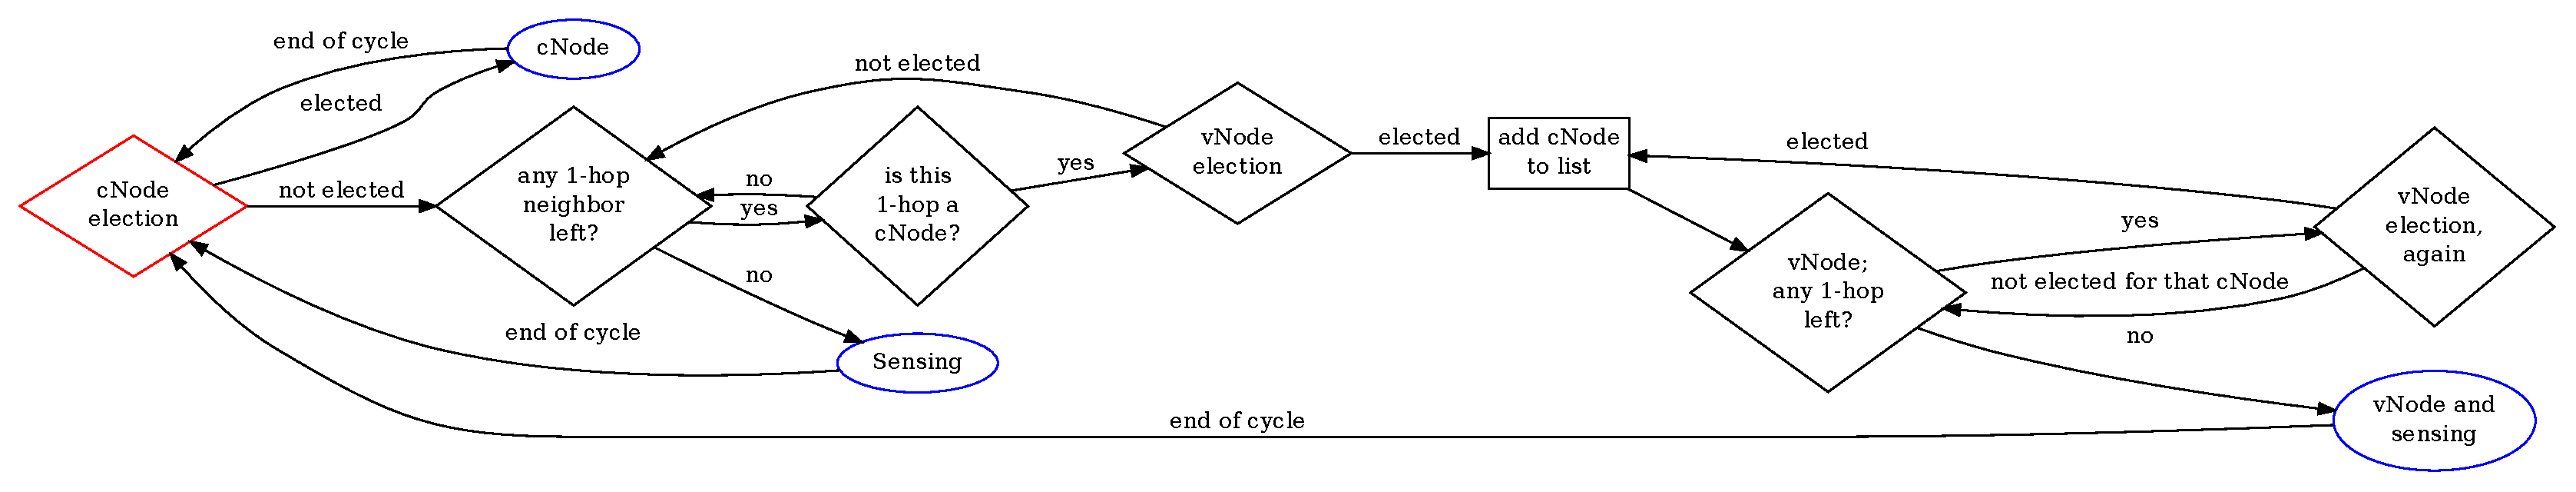
\includegraphics[width=\textwidth]{\chapterfig/state_graph.eps}
    \caption{State machine of the (non-\CH) nodes}\label{se:fig:states}
\end{figure*}

    \subsection{Cluster coverage in case of heterogeneous activity}

Deterministic election of the \cns does not only introduce a flaw that compromised nodes could try to exploit.
There is a second problem, independent from the nodes behavior, that could prevent the detection of compromised nodes.
If a region of the network happens to produce more traffic activity than the other parts of the network, the energy of its nodes will be drawn faster.
In consequence, none of the $n$ nodes with the highest residual energy ($n$ being the desired number of \cns during each cycle) will be located inside this region, and some nodes may not be covered for surveillance as long as traffic do not fade, possibly for all cycles.
\figurename~\ref{se:fig:cover} illustrates this problem.
\begin{figure}[h]
    \centering
    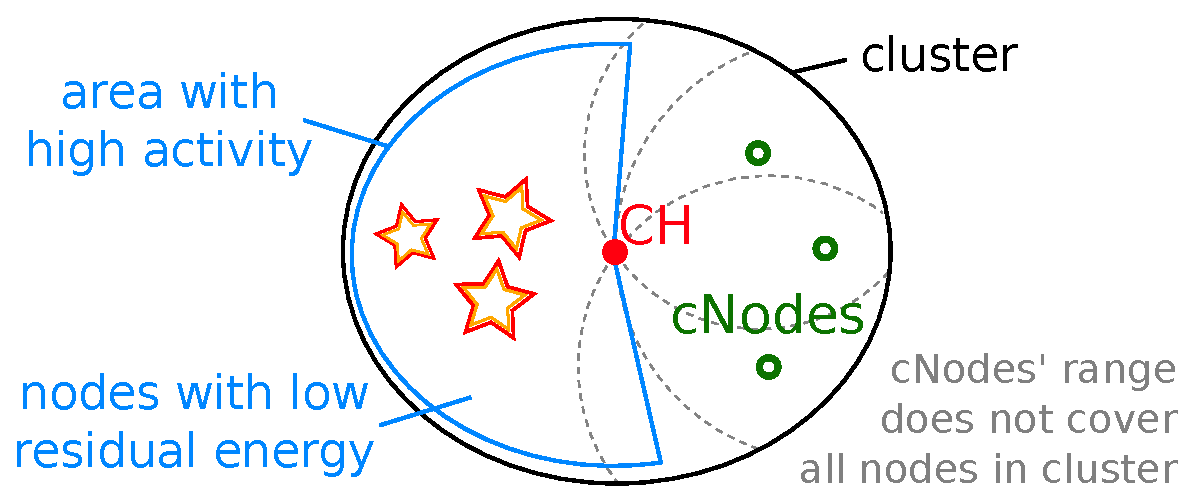
\includegraphics[width=.8\linewidth]{\chapterfig/cover.eps}
    \caption{Illustrative scheme: \cns are elected inside the area with less activity (thus with more residual energy) and do not cover nodes from the opposite side of the network.}\label{se:fig:cover}
\end{figure}

To address this issue we need to ensure that every node in the network is covered by at least one \cn.
So the election process we presented in~\ref{se:subsubsec:elec1} needs to be modified.
The correct version is as follows:

\begin{enumerate}
    \item During first step, each node evaluates its residual energy and broadcasts the value;
    \item The \ch listens to all values. Other nodes also register all messages they hear into memory;
    \item All nodes send to the \CH the list of their 1-hop neighbors\footnote{We do not deal with the case of compromised nodes cheating at this step of the process. Indeed they could announce extra virtual neighbors to try to escape from coverage.};
    \item The \CH picks the $n$ nodes among those with the highest residual energy, such that the $n$ nodes cover all other nodes in range\footnote{The details of the algorithm executed by the \ch at this step are not given in this study.}. If needed, it selects some additional nodes to cover all the cluster;
    \item The \CH returns to selected nodes a message to assign them the role of \cn.
\end{enumerate}

Note that some clustering algorithms (such as HEED~\cite{YF04} for example) provide other election mechanisms (for \chs, but that can also be used for selecting \cns) based on residual energy.
We do not want to use it because energy only takes part in the process as a factor for probability that the nodes declare themselves elected.
Instead we prefer nodes to broadcast their residual energy in order to enable surveillance by the \vns.

    \subsection{Observations}

\cns apply a very basic trust based scheme to the cluster: when a sensor node breaks a rule, for example by exceeding a given threshold for transmitted packets, it is considered as untrustworthy.
There are many other trust based schemes in literature, most of them more advanced than this one (see Section~\ref{se:sec:related}).
The \cns could implement several other trust mechanisms (by lowering a score on bad behaviour for each node for instance).
As more complex mechanism would create additional overhead, we prefer to limit to this simple method in this study.
%%%%%%%%%%%%%%%%%%%%%%%%%%%%%%%%%%%%%%%%%%%%%%%%%%%%%%%%%%%%%%%%%%%%%%%%%%%%%%%%%%%%%%
%%%%%%%%%%%%%%%%%%%%%%%%%%%%%%%%%%%%%%%%%%%%%%%%%%%%%%%%%%%%%%%%%%%%%%%%%%%%%%%%%%%%%%
%A first observation relates to overall complexity of the \cns election process.
%The proposed solution consists in the designation of nodes monitoring the monitors.
%The \vn role is a new role we introduce in the paper.
%It comes with a heavier election algorithm which make each node in the cluster send broadcast messages during the process (to announce residual energy and the list of direct neighbors).
%It is obvious that algorithmic complexity is increased, and that the system is heavier to implement than a simple pseudo-random election for the \cns.
%
%Along with overall complexity, overhead is also increased.
%Both those factors impact the nodes consumption.
%Note that we do not seek to decrease the comprehensive consumption of energy in the network; instead, we try to improve load balancing in order to keep alive as many nodes in the cluster as we can as time goes by.
%
%Another point not related to complexity is also worthy of interest: the use of \cns and \vns does not ensure a perfect guaranty of security.
%This system relies on several hypotheses, such as the fact that compromised nodes do not collaborate between them:
%a compromised node being elected as \cn could for instance announce to the \CH, during the election, that he can reach and survey some areas in the cluster, in order to make the \CH believe the area is surveyed (while in fact even the rogue \cn might not reach it).
%If the \CH does not assign other \cn to watch over this area, some other compromised nodes may go undetected and attack the network.
%
%The second hypothesis to note is that the proposed solution currently assumes that the \ch is not compromised.
